\chapter{Implementation}
\label{chap:implementation}

This chapter presents an in-depth description of how \f{} works
and demonstrates how much it can simplify developers' experience
by showing a real-world example with an extensive usage of its features.
Furthermore, since we are creating an open-source project, the structure of
the repository will also be analyzed.


\section{Overview}

\f{} is a transpiler which enhances serverless programming by introducing the concept of annotations.
Annotations are an abstraction layer that the developers can unobtrusively use
to apply code transformations and metadata generation to a given application,
which will be deployed to a serverless platform.

To achieve this goal, we used the \textit{TypeScript}\cite{ts} compiler API which lets us
manipulate sources with ease, and \textit{SLS}\cite{sls} which
uses the generated metadata to deploy to \textit{AWS Lambda}.

\begin{figure}[H]
  \centering
  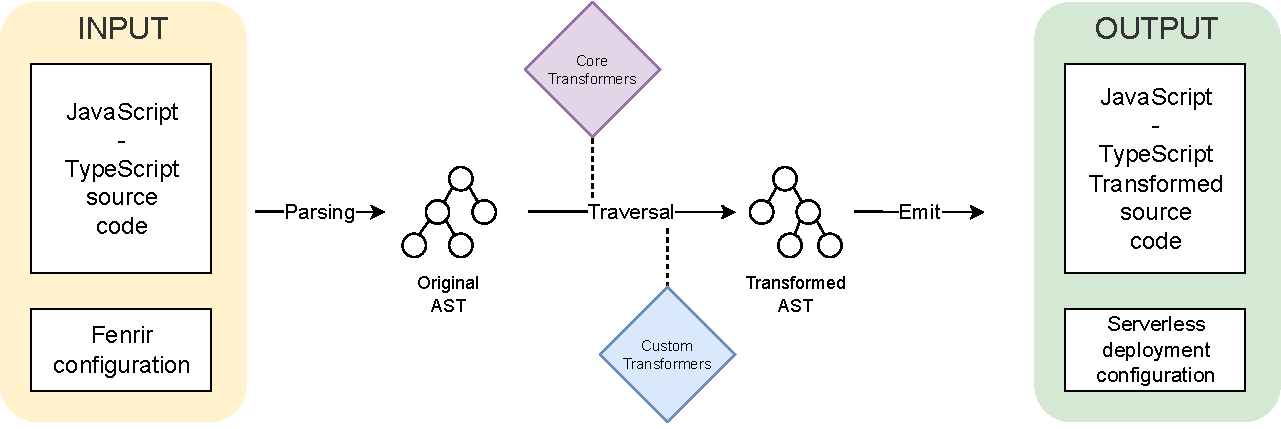
\includegraphics[width=\textwidth]{diagrams/pipeline}
  \caption{Transpiler pipeline.}
  \label{fig:pipeline}
\end{figure}


The transpilation pipeline, depicted in Figure \ref{fig:pipeline},
starts with the parsing of the input source code, which produces AST nodes with their related
annotations. Then, each annotation induces the application of its related
transformation step, whose output is fed into the next transformer, if any.
During the transformation steps, \f{} reports possible errors by gracefully
stopping the compilation process and indicating the offending instructions. Once
the transformations have taken place without any errors, the output code is saved
and the related metadata is also appended to a
\verb|serverless.yml| file which specifies function deployment
properties (e.g., the address to invoke a given function).

\subsection{Brief example of a Monolith to Serverless compilation}

The following brief example should\dots
